\title{Higher-Order Derivatives and Smoothness}
\documentclass{article}
\author{Aidan Ewart}
\date{\today}

\usepackage{graphicx}
\graphicspath{{./images}}

\usepackage{amsmath}

\begin{document}
\maketitle

It might be useful to formally define the intuitive notion of `smoothness' for real functions.
Intuitively, one might assume that continuity is a sufficient condition; a continuous function
contains no sudden jumps which would surely prevent it from being considered smooth in any
reasonable sense. However, the existence of functions such as the Weierstrass function, which
would certainly not be considered smooth, and yet is still continuous, show that a stronger
condition is required:
\\\\
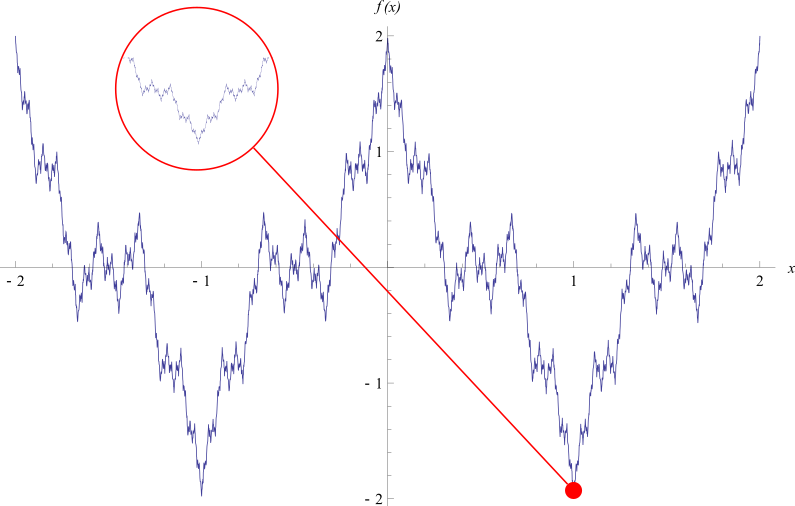
\includegraphics[width=\textwidth]{WeierstrassFunction.png}
\\\\
We may use the derivative operation to define a stronger condition for smoothness. We say
that a function is \emph{differentiable} iff the derivative is defined at every point in the
domain of the function. For example, $\ln(x)$ is differentiable, even though the derivative
is not defined at $x \leq 0$, as $x \leq 0$ is not in the domain of $\ln(x)$.
\\\\
TODO: IMAGE OF $ln(x)$ and $x^{-1}$
\\\\
It seems that differentiability might be a good candidate for a definition of smoothness.
However, consider the function:
$$
f(x) = \left\{ \begin{array}{ll}
    x^2 \sin(\frac{1}{x}) & \mbox{if } x \neq 0 \\
    0 & \mbox{if } x = 0
\end{array} \right.
$$
The derivative of this function clearly exists at all points $x \neq 0$, and indeed we can
show the derivative exists at $x=0$ using the limit definition of the derivative:
\begin{align*}
f'(x) & = \lim_{h \to 0} \frac{f(x+h) - f(x)}{h}
\\
f'(0) & = \lim_{h \to 0} \frac{h^2 \sin(\frac{1}{h}) - f(0)}{h}
\\
f'(0) & = \lim_{h \to 0} \frac{h^2 \sin(\frac{1}{h}) - 0}{h}
\\
& = \lim_{h \to 0} h \sin(\frac{1}{h})
\\
& = 0
\end{align*}
However, the function might not be considered smooth, as it gets arbitrarily `rough' as we
approach $x=0$:
\\\\
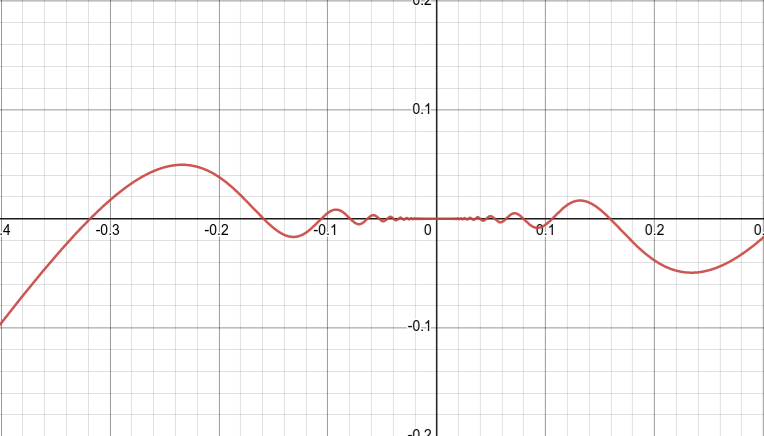
\includegraphics[width=\textwidth]{discon_deriv.png}
\\\\
It turns out that $f'(x)$ is actually discontinuous [EXPAND UPON - GIVE DEFINITION OF CONTINUITY].
\end{document}